\documentclass[twoside]{book}

% Packages required by doxygen
\usepackage{fixltx2e}
\usepackage{calc}
\usepackage{doxygen}
\usepackage[export]{adjustbox} % also loads graphicx
\usepackage{graphicx}
\usepackage[utf8]{inputenc}
\usepackage{makeidx}
\usepackage{multicol}
\usepackage{multirow}
\PassOptionsToPackage{warn}{textcomp}
\usepackage{textcomp}
\usepackage[nointegrals]{wasysym}
\usepackage[table]{xcolor}

% Font selection
\usepackage[T1]{fontenc}
\usepackage[scaled=.90]{helvet}
\usepackage{courier}
\usepackage{amssymb}
\usepackage{sectsty}
\renewcommand{\familydefault}{\sfdefault}
\allsectionsfont{%
  \fontseries{bc}\selectfont%
  \color{darkgray}%
}
\renewcommand{\DoxyLabelFont}{%
  \fontseries{bc}\selectfont%
  \color{darkgray}%
}
\newcommand{\+}{\discretionary{\mbox{\scriptsize$\hookleftarrow$}}{}{}}

% Page & text layout
\usepackage{geometry}
\geometry{%
  a4paper,%
  top=2.5cm,%
  bottom=2.5cm,%
  left=2.5cm,%
  right=2.5cm%
}
\tolerance=750
\hfuzz=15pt
\hbadness=750
\setlength{\emergencystretch}{15pt}
\setlength{\parindent}{0cm}
\setlength{\parskip}{3ex plus 2ex minus 2ex}
\makeatletter
\renewcommand{\paragraph}{%
  \@startsection{paragraph}{4}{0ex}{-1.0ex}{1.0ex}{%
    \normalfont\normalsize\bfseries\SS@parafont%
  }%
}
\renewcommand{\subparagraph}{%
  \@startsection{subparagraph}{5}{0ex}{-1.0ex}{1.0ex}{%
    \normalfont\normalsize\bfseries\SS@subparafont%
  }%
}
\makeatother

% Headers & footers
\usepackage{fancyhdr}
\pagestyle{fancyplain}
\fancyhead[LE]{\fancyplain{}{\bfseries\thepage}}
\fancyhead[CE]{\fancyplain{}{}}
\fancyhead[RE]{\fancyplain{}{\bfseries\leftmark}}
\fancyhead[LO]{\fancyplain{}{\bfseries\rightmark}}
\fancyhead[CO]{\fancyplain{}{}}
\fancyhead[RO]{\fancyplain{}{\bfseries\thepage}}
\fancyfoot[LE]{\fancyplain{}{}}
\fancyfoot[CE]{\fancyplain{}{}}
\fancyfoot[RE]{\fancyplain{}{\bfseries\scriptsize Generated by Doxygen }}
\fancyfoot[LO]{\fancyplain{}{\bfseries\scriptsize Generated by Doxygen }}
\fancyfoot[CO]{\fancyplain{}{}}
\fancyfoot[RO]{\fancyplain{}{}}
\renewcommand{\footrulewidth}{0.4pt}
\renewcommand{\chaptermark}[1]{%
  \markboth{#1}{}%
}
\renewcommand{\sectionmark}[1]{%
  \markright{\thesection\ #1}%
}

% Indices & bibliography
\usepackage{natbib}
\usepackage[titles]{tocloft}
\setcounter{tocdepth}{3}
\setcounter{secnumdepth}{5}
\makeindex

% Hyperlinks (required, but should be loaded last)
\usepackage{ifpdf}
\ifpdf
  \usepackage[pdftex,pagebackref=true]{hyperref}
\else
  \usepackage[ps2pdf,pagebackref=true]{hyperref}
\fi
\hypersetup{%
  colorlinks=true,%
  linkcolor=blue,%
  citecolor=blue,%
  unicode%
}

% Custom commands
\newcommand{\clearemptydoublepage}{%
  \newpage{\pagestyle{empty}\cleardoublepage}%
}

\usepackage{caption}
\captionsetup{labelsep=space,justification=centering,font={bf},singlelinecheck=off,skip=4pt,position=top}

%===== C O N T E N T S =====

\begin{document}

% Titlepage & ToC
\hypersetup{pageanchor=false,
             bookmarksnumbered=true,
             pdfencoding=unicode
            }
\pagenumbering{roman}
\begin{titlepage}
\vspace*{7cm}
\begin{center}%
{\Large U\+Iwithout\+QT \\[1ex]\large 1.\+00 }\\
\vspace*{1cm}
{\large Generated by Doxygen 1.8.11}\\
\end{center}
\end{titlepage}
\clearemptydoublepage
\tableofcontents
\clearemptydoublepage
\pagenumbering{arabic}
\hypersetup{pageanchor=true}

%--- Begin generated contents ---
\chapter{Hierarchical Index}
\section{Class Hierarchy}
This inheritance list is sorted roughly, but not completely, alphabetically\+:\begin{DoxyCompactList}
\item \contentsline{section}{Camera}{\pageref{class_camera}}{}
\item \contentsline{section}{Cm\+Shape\+Context}{\pageref{class_cm_shape_context}}{}
\item \contentsline{section}{Colour}{\pageref{struct_colour}}{}
\item \contentsline{section}{Display}{\pageref{class_display}}{}
\item \contentsline{section}{Element}{\pageref{struct_element}}{}
\item \contentsline{section}{Indexed\+Model}{\pageref{class_indexed_model}}{}
\item \contentsline{section}{Material}{\pageref{struct_material}}{}
\item \contentsline{section}{Mesh}{\pageref{class_mesh}}{}
\item \contentsline{section}{O\+B\+J\+Index}{\pageref{struct_o_b_j_index}}{}
\item \contentsline{section}{O\+B\+J\+Model}{\pageref{class_o_b_j_model}}{}
\item \contentsline{section}{Shader}{\pageref{class_shader}}{}
\item \contentsline{section}{Silhouette\+Data}{\pageref{struct_silhouette_data}}{}
\item \contentsline{section}{Similarity\+Evaluator}{\pageref{class_similarity_evaluator}}{}
\item \contentsline{section}{Transform}{\pageref{class_transform}}{}
\item vector\begin{DoxyCompactList}
\item \contentsline{section}{D\+B\+\_\+elements}{\pageref{class_d_b__elements}}{}
\end{DoxyCompactList}
\item \contentsline{section}{Vertex}{\pageref{class_vertex}}{}
\end{DoxyCompactList}

\chapter{Class Index}
\section{Class List}
Here are the classes, structs, unions and interfaces with brief descriptions\+:\begin{DoxyCompactList}
\item\contentsline{section}{\hyperlink{class_camera}{Camera} }{\pageref{class_camera}}{}
\item\contentsline{section}{\hyperlink{class_cm_shape_context}{Cm\+Shape\+Context} }{\pageref{class_cm_shape_context}}{}
\item\contentsline{section}{\hyperlink{struct_colour}{Colour} }{\pageref{struct_colour}}{}
\item\contentsline{section}{\hyperlink{class_d_b__elements}{D\+B\+\_\+elements} }{\pageref{class_d_b__elements}}{}
\item\contentsline{section}{\hyperlink{class_display}{Display} }{\pageref{class_display}}{}
\item\contentsline{section}{\hyperlink{struct_element}{Element} }{\pageref{struct_element}}{}
\item\contentsline{section}{\hyperlink{class_indexed_model}{Indexed\+Model} }{\pageref{class_indexed_model}}{}
\item\contentsline{section}{\hyperlink{struct_material}{Material} }{\pageref{struct_material}}{}
\item\contentsline{section}{\hyperlink{class_mesh}{Mesh} }{\pageref{class_mesh}}{}
\item\contentsline{section}{\hyperlink{struct_o_b_j_index}{O\+B\+J\+Index} }{\pageref{struct_o_b_j_index}}{}
\item\contentsline{section}{\hyperlink{class_o_b_j_model}{O\+B\+J\+Model} }{\pageref{class_o_b_j_model}}{}
\item\contentsline{section}{\hyperlink{class_shader}{Shader} }{\pageref{class_shader}}{}
\item\contentsline{section}{\hyperlink{struct_silhouette_data}{Silhouette\+Data} }{\pageref{struct_silhouette_data}}{}
\item\contentsline{section}{\hyperlink{class_similarity_evaluator}{Similarity\+Evaluator} }{\pageref{class_similarity_evaluator}}{}
\item\contentsline{section}{\hyperlink{class_transform}{Transform} }{\pageref{class_transform}}{}
\item\contentsline{section}{\hyperlink{class_vertex}{Vertex} }{\pageref{class_vertex}}{}
\end{DoxyCompactList}

\chapter{Class Documentation}
\hypertarget{class_camera}{}\section{Camera Class Reference}
\label{class_camera}\index{Camera@{Camera}}


Collaboration diagram for Camera\+:
\nopagebreak
\begin{figure}[H]
\begin{center}
\leavevmode
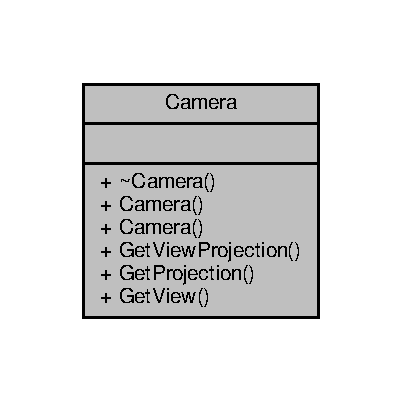
\includegraphics[width=193pt]{class_camera__coll__graph}
\end{center}
\end{figure}
\subsection*{Public Member Functions}
\begin{DoxyCompactItemize}
\item 
{\bfseries Camera} (const \hyperlink{class_mesh}{Mesh} \&mesh, float fov, float aspect, float z\+Near, float z\+Far)\hypertarget{class_camera_ace593335719e93de3737f5198fc6d61e}{}\label{class_camera_ace593335719e93de3737f5198fc6d61e}

\item 
{\bfseries Camera} (glm\+::vec3 pos, const \hyperlink{class_mesh}{Mesh} \&mesh, float aspect, glm\+::vec3 up)\hypertarget{class_camera_adca502e8d99559c3e15d224c826d482c}{}\label{class_camera_adca502e8d99559c3e15d224c826d482c}

\item 
glm\+::mat4 {\bfseries Get\+View\+Projection} () const \hypertarget{class_camera_a7ab7d6e30a473392949f993856b14517}{}\label{class_camera_a7ab7d6e30a473392949f993856b14517}

\item 
glm\+::mat4 {\bfseries Get\+Projection} () const \hypertarget{class_camera_adb63c52b3975a50b512761317758b830}{}\label{class_camera_adb63c52b3975a50b512761317758b830}

\item 
glm\+::mat4 {\bfseries Get\+View} () const \hypertarget{class_camera_aca3834159d8421515e96c9e00e8d2e7b}{}\label{class_camera_aca3834159d8421515e96c9e00e8d2e7b}

\end{DoxyCompactItemize}


The documentation for this class was generated from the following files\+:\begin{DoxyCompactItemize}
\item 
camera.\+h\item 
camera.\+cpp\end{DoxyCompactItemize}

\hypertarget{class_cm_shape_context}{}\section{Cm\+Shape\+Context Class Reference}
\label{class_cm_shape_context}\index{Cm\+Shape\+Context@{Cm\+Shape\+Context}}


Collaboration diagram for Cm\+Shape\+Context\+:\nopagebreak
\begin{figure}[H]
\begin{center}
\leavevmode
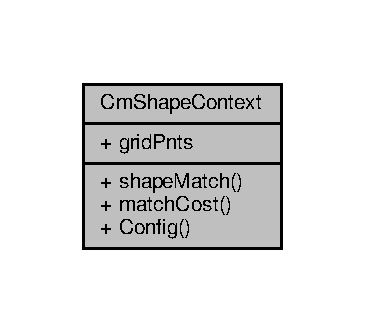
\includegraphics[width=175pt]{class_cm_shape_context__coll__graph}
\end{center}
\end{figure}
\subsection*{Public Member Functions}
\begin{DoxyCompactItemize}
\item 
double {\bfseries shape\+Match} (Point\+Setd \&pnt\+Set1, Point\+Setd \&pnt\+Set2, double \&sc\+Cost, double \&aff\+Cost)\hypertarget{class_cm_shape_context_a27acc09496f499ba714176074259f475}{}\label{class_cm_shape_context_a27acc09496f499ba714176074259f475}

\item 
double {\bfseries match\+Cost} (Point\+Setd \&pnt\+Set1, Point\+Setd \&pnt\+Set2, double wsc=0.\+95)\hypertarget{class_cm_shape_context_aa45ed20b3c9389de2d0d8cb0b1db3eab}{}\label{class_cm_shape_context_aa45ed20b3c9389de2d0d8cb0b1db3eab}

\end{DoxyCompactItemize}
\subsection*{Static Public Member Functions}
\begin{DoxyCompactItemize}
\item 
static void {\bfseries Config} (bool display=false, int iters=1, double dummy\+Fraction=0.\+25)\hypertarget{class_cm_shape_context_a5f77b1ed0749126d4d287941b00e5ef6}{}\label{class_cm_shape_context_a5f77b1ed0749126d4d287941b00e5ef6}

\end{DoxyCompactItemize}
\subsection*{Public Attributes}
\begin{DoxyCompactItemize}
\item 
Point\+Setd {\bfseries grid\+Pnts}\hypertarget{class_cm_shape_context_aeeec0906d70a3209d7eba947661d8409}{}\label{class_cm_shape_context_aeeec0906d70a3209d7eba947661d8409}

\end{DoxyCompactItemize}


The documentation for this class was generated from the following files\+:\begin{DoxyCompactItemize}
\item 
cmshapecontext.\+h\item 
cmshapecontext.\+cpp\end{DoxyCompactItemize}

\hypertarget{struct_colour}{}\section{Colour Struct Reference}
\label{struct_colour}\index{Colour@{Colour}}


Collaboration diagram for Colour\+:\nopagebreak
\begin{figure}[H]
\begin{center}
\leavevmode
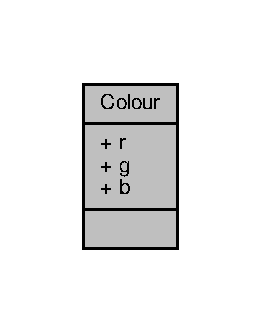
\includegraphics[width=125pt]{struct_colour__coll__graph}
\end{center}
\end{figure}
\subsection*{Public Attributes}
\begin{DoxyCompactItemize}
\item 
float {\bfseries r}\hypertarget{struct_colour_acb0b39e6e5e18b946732f51f126c8bf8}{}\label{struct_colour_acb0b39e6e5e18b946732f51f126c8bf8}

\item 
float {\bfseries g}\hypertarget{struct_colour_a25bdab33ddd5f646162329bfb8b23b75}{}\label{struct_colour_a25bdab33ddd5f646162329bfb8b23b75}

\item 
float {\bfseries b}\hypertarget{struct_colour_aee312356ce76f9c54c9beecad919b421}{}\label{struct_colour_aee312356ce76f9c54c9beecad919b421}

\end{DoxyCompactItemize}


The documentation for this struct was generated from the following file\+:\begin{DoxyCompactItemize}
\item 
material.\+h\end{DoxyCompactItemize}

\hypertarget{class_d_b__elements}{}\section{D\+B\+\_\+elements Class Reference}
\label{class_d_b__elements}\index{D\+B\+\_\+elements@{D\+B\+\_\+elements}}


Inheritance diagram for D\+B\+\_\+elements\+:\nopagebreak
\begin{figure}[H]
\begin{center}
\leavevmode
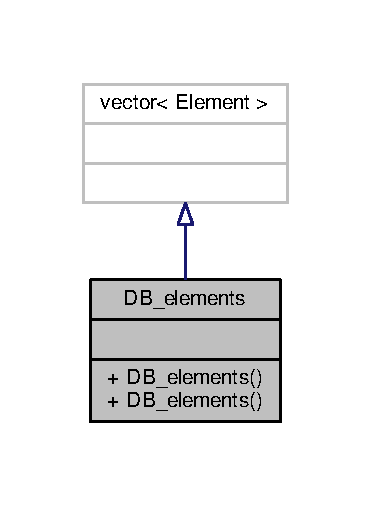
\includegraphics[width=178pt]{class_d_b__elements__inherit__graph}
\end{center}
\end{figure}


Collaboration diagram for D\+B\+\_\+elements\+:\nopagebreak
\begin{figure}[H]
\begin{center}
\leavevmode
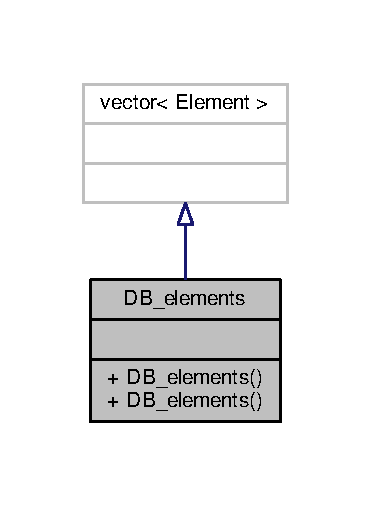
\includegraphics[width=178pt]{class_d_b__elements__coll__graph}
\end{center}
\end{figure}
\subsection*{Public Member Functions}
\begin{DoxyCompactItemize}
\item 
{\bfseries D\+B\+\_\+elements} (const string \&file\+Name, const int C\+A\+N\+D\+I\+D\+A\+T\+E\+\_\+\+P\+O\+I\+N\+TS)\hypertarget{class_d_b__elements_a1e648b5c8b7fcad6455e6d93e7530c4e}{}\label{class_d_b__elements_a1e648b5c8b7fcad6455e6d93e7530c4e}

\end{DoxyCompactItemize}


The documentation for this class was generated from the following files\+:\begin{DoxyCompactItemize}
\item 
db\+\_\+elements.\+h\item 
db\+\_\+elements.\+cpp\end{DoxyCompactItemize}

\hypertarget{class_display}{}\section{Display Class Reference}
\label{class_display}\index{Display@{Display}}


Collaboration diagram for Display\+:\nopagebreak
\begin{figure}[H]
\begin{center}
\leavevmode
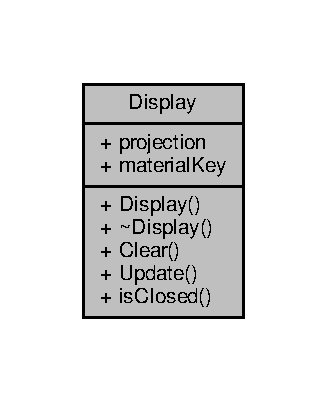
\includegraphics[width=157pt]{class_display__coll__graph}
\end{center}
\end{figure}
\subsection*{Public Types}
\begin{DoxyCompactItemize}
\item 
enum {\bfseries projection\+Type} \{ {\bfseries P\+E\+R\+S\+P\+E\+C\+T\+I\+V\+E\+\_\+P}, 
{\bfseries O\+R\+T\+H\+O\+G\+R\+A\+P\+H\+I\+C\+\_\+P}
 \}\hypertarget{class_display_a3ba4e50bfd82272df6f4d6b7ff930502}{}\label{class_display_a3ba4e50bfd82272df6f4d6b7ff930502}

\end{DoxyCompactItemize}
\subsection*{Public Member Functions}
\begin{DoxyCompactItemize}
\item 
{\bfseries Display} (int width, int height, const std\+::string \&title)\hypertarget{class_display_a87a6f6c52cfc4ba3be9ad262ab3d45a5}{}\label{class_display_a87a6f6c52cfc4ba3be9ad262ab3d45a5}

\item 
void {\bfseries Clear} (float r, float g, float b, float a)\hypertarget{class_display_a8681db3f75e07bc3df838c0a33de8472}{}\label{class_display_a8681db3f75e07bc3df838c0a33de8472}

\item 
void {\bfseries Update} (\hyperlink{class_transform}{Transform} \&transform\+\_\+camera, \hyperlink{class_transform}{Transform} \&transform\+\_\+\+O\+BB)\hypertarget{class_display_ab872805f73a9521c7e4e646404d8a0b4}{}\label{class_display_ab872805f73a9521c7e4e646404d8a0b4}

\item 
bool {\bfseries is\+Closed} ()\hypertarget{class_display_ad72eae29139375a697766d9fb1450a38}{}\label{class_display_ad72eae29139375a697766d9fb1450a38}

\end{DoxyCompactItemize}
\subsection*{Public Attributes}
\begin{DoxyCompactItemize}
\item 
bool {\bfseries projection}\hypertarget{class_display_a9167af31dc8fc8771c9c202d428f6196}{}\label{class_display_a9167af31dc8fc8771c9c202d428f6196}

\item 
int {\bfseries material\+Key}\hypertarget{class_display_a6ad25732b6e448b26b04bafec5930b7e}{}\label{class_display_a6ad25732b6e448b26b04bafec5930b7e}

\end{DoxyCompactItemize}


The documentation for this class was generated from the following files\+:\begin{DoxyCompactItemize}
\item 
display.\+h\item 
display.\+cpp\end{DoxyCompactItemize}

\hypertarget{struct_element}{}\section{Element Struct Reference}
\label{struct_element}\index{Element@{Element}}


Collaboration diagram for Element\+:\nopagebreak
\begin{figure}[H]
\begin{center}
\leavevmode
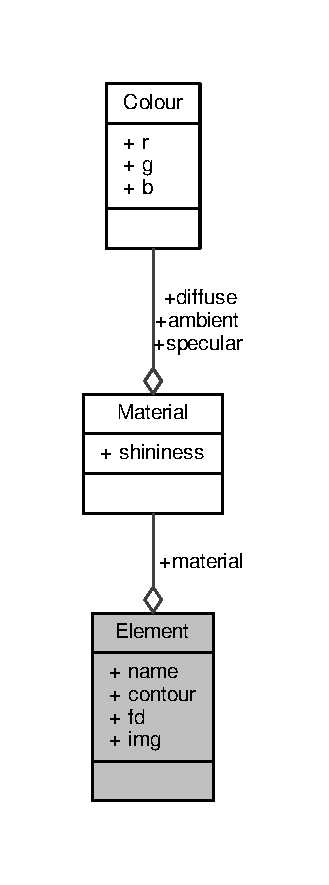
\includegraphics[width=158pt]{struct_element__coll__graph}
\end{center}
\end{figure}
\subsection*{Public Attributes}
\begin{DoxyCompactItemize}
\item 
string {\bfseries name}\hypertarget{struct_element_a63e156c168905a24437098bfff0e5366}{}\label{struct_element_a63e156c168905a24437098bfff0e5366}

\item 
vector$<$ Point2d $>$ {\bfseries contour}\hypertarget{struct_element_a891d67998b628871128c79048edbdca6}{}\label{struct_element_a891d67998b628871128c79048edbdca6}

\item 
\hyperlink{struct_material}{Material} {\bfseries material}\hypertarget{struct_element_ab4734353ea9dba55cd3cadbff0053bfb}{}\label{struct_element_ab4734353ea9dba55cd3cadbff0053bfb}

\item 
vector$<$ complex$<$ float $>$ $>$ {\bfseries fd}\hypertarget{struct_element_a0ed928b41b1f11516f3130d271d6b7e4}{}\label{struct_element_a0ed928b41b1f11516f3130d271d6b7e4}

\item 
Mat {\bfseries img}\hypertarget{struct_element_adbe2265fc367b0e01241b9d779b04f47}{}\label{struct_element_adbe2265fc367b0e01241b9d779b04f47}

\end{DoxyCompactItemize}


The documentation for this struct was generated from the following file\+:\begin{DoxyCompactItemize}
\item 
db\+\_\+elements.\+h\end{DoxyCompactItemize}

\hypertarget{class_indexed_model}{}\section{Indexed\+Model Class Reference}
\label{class_indexed_model}\index{Indexed\+Model@{Indexed\+Model}}


Collaboration diagram for Indexed\+Model\+:\nopagebreak
\begin{figure}[H]
\begin{center}
\leavevmode
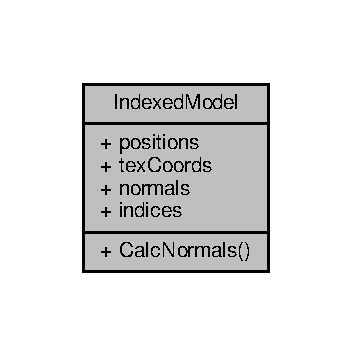
\includegraphics[width=169pt]{class_indexed_model__coll__graph}
\end{center}
\end{figure}
\subsection*{Public Member Functions}
\begin{DoxyCompactItemize}
\item 
void {\bfseries Calc\+Normals} ()\hypertarget{class_indexed_model_ad7c6f8680a079108e64d463b34dca802}{}\label{class_indexed_model_ad7c6f8680a079108e64d463b34dca802}

\end{DoxyCompactItemize}
\subsection*{Public Attributes}
\begin{DoxyCompactItemize}
\item 
std\+::vector$<$ glm\+::vec3 $>$ {\bfseries positions}\hypertarget{class_indexed_model_a81d6b9180bd152add38881ed6def521a}{}\label{class_indexed_model_a81d6b9180bd152add38881ed6def521a}

\item 
std\+::vector$<$ glm\+::vec2 $>$ {\bfseries tex\+Coords}\hypertarget{class_indexed_model_a8b7d3dd202865fb909f6cc07080f0f8d}{}\label{class_indexed_model_a8b7d3dd202865fb909f6cc07080f0f8d}

\item 
std\+::vector$<$ glm\+::vec3 $>$ {\bfseries normals}\hypertarget{class_indexed_model_a43a9aa25e0461c1a729693fd7efaf45f}{}\label{class_indexed_model_a43a9aa25e0461c1a729693fd7efaf45f}

\item 
std\+::vector$<$ unsigned int $>$ {\bfseries indices}\hypertarget{class_indexed_model_ae9ab23aa197180acd72e017503dd6a34}{}\label{class_indexed_model_ae9ab23aa197180acd72e017503dd6a34}

\end{DoxyCompactItemize}


The documentation for this class was generated from the following files\+:\begin{DoxyCompactItemize}
\item 
obj\+\_\+loader.\+h\item 
obj\+\_\+loader.\+cpp\end{DoxyCompactItemize}

\hypertarget{struct_material}{}\section{Material Struct Reference}
\label{struct_material}\index{Material@{Material}}


Collaboration diagram for Material\+:\nopagebreak
\begin{figure}[H]
\begin{center}
\leavevmode
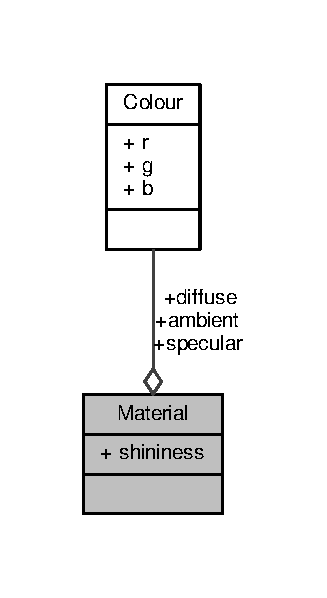
\includegraphics[width=157pt]{struct_material__coll__graph}
\end{center}
\end{figure}
\subsection*{Public Attributes}
\begin{DoxyCompactItemize}
\item 
\hyperlink{struct_colour}{Colour} {\bfseries ambient}\hypertarget{struct_material_a6946c65f77b05aa25bb92eaffa7b87c9}{}\label{struct_material_a6946c65f77b05aa25bb92eaffa7b87c9}

\item 
\hyperlink{struct_colour}{Colour} {\bfseries diffuse}\hypertarget{struct_material_a87015a28f42c846ccf0f8d1637f20988}{}\label{struct_material_a87015a28f42c846ccf0f8d1637f20988}

\item 
\hyperlink{struct_colour}{Colour} {\bfseries specular}\hypertarget{struct_material_a95cd1427d513fdf9220053fdd709e390}{}\label{struct_material_a95cd1427d513fdf9220053fdd709e390}

\item 
float {\bfseries shininess}\hypertarget{struct_material_a9dc184c883ec135ace28c1917af3fe84}{}\label{struct_material_a9dc184c883ec135ace28c1917af3fe84}

\end{DoxyCompactItemize}


The documentation for this struct was generated from the following file\+:\begin{DoxyCompactItemize}
\item 
material.\+h\end{DoxyCompactItemize}

\hypertarget{class_mesh}{}\section{Mesh Class Reference}
\label{class_mesh}\index{Mesh@{Mesh}}


Collaboration diagram for Mesh\+:\nopagebreak
\begin{figure}[H]
\begin{center}
\leavevmode
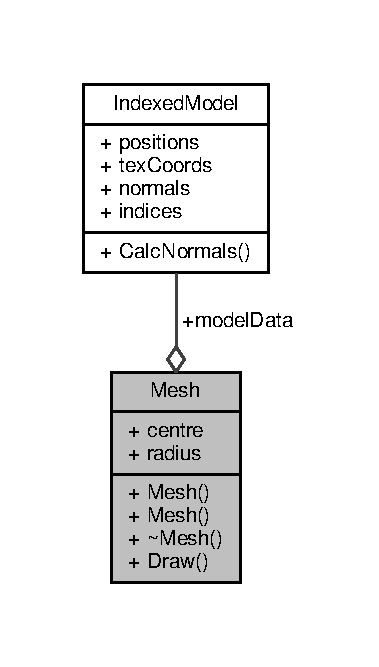
\includegraphics[width=182pt]{class_mesh__coll__graph}
\end{center}
\end{figure}
\subsection*{Public Member Functions}
\begin{DoxyCompactItemize}
\item 
{\bfseries Mesh} (const std\+::string \&file\+Name)\hypertarget{class_mesh_a4c4a1abe6f54d0bc2e4d07908fa43f21}{}\label{class_mesh_a4c4a1abe6f54d0bc2e4d07908fa43f21}

\item 
{\bfseries Mesh} (\hyperlink{class_vertex}{Vertex} $\ast$vertices, unsigned int num\+Vertices, unsigned int $\ast$indices, unsigned int num\+Indices)\hypertarget{class_mesh_a2401dd4fde4e5dbce58b5964648051e2}{}\label{class_mesh_a2401dd4fde4e5dbce58b5964648051e2}

\item 
void {\bfseries Draw} ()\hypertarget{class_mesh_afdd95c079fd0442afef8a6c421c8bfc9}{}\label{class_mesh_afdd95c079fd0442afef8a6c421c8bfc9}

\end{DoxyCompactItemize}
\subsection*{Public Attributes}
\begin{DoxyCompactItemize}
\item 
glm\+::vec3 {\bfseries centre}\hypertarget{class_mesh_a2416d7b5352e7278ad988652ad144456}{}\label{class_mesh_a2416d7b5352e7278ad988652ad144456}

\item 
float {\bfseries radius}\hypertarget{class_mesh_a5fc0e801c0a883e0b759dcc380f20144}{}\label{class_mesh_a5fc0e801c0a883e0b759dcc380f20144}

\item 
\hyperlink{class_indexed_model}{Indexed\+Model} {\bfseries model\+Data}\hypertarget{class_mesh_a40c3a6a03dd76f1856abce53948919c5}{}\label{class_mesh_a40c3a6a03dd76f1856abce53948919c5}

\end{DoxyCompactItemize}


The documentation for this class was generated from the following files\+:\begin{DoxyCompactItemize}
\item 
mesh.\+h\item 
mesh.\+cpp\end{DoxyCompactItemize}

\hypertarget{struct_o_b_j_index}{}\section{O\+B\+J\+Index Struct Reference}
\label{struct_o_b_j_index}\index{O\+B\+J\+Index@{O\+B\+J\+Index}}


Collaboration diagram for O\+B\+J\+Index\+:\nopagebreak
\begin{figure}[H]
\begin{center}
\leavevmode
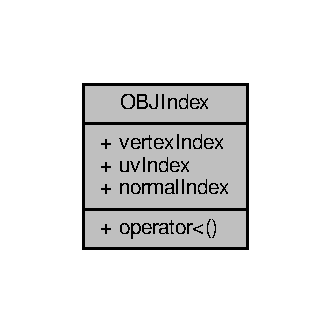
\includegraphics[width=159pt]{struct_o_b_j_index__coll__graph}
\end{center}
\end{figure}
\subsection*{Public Member Functions}
\begin{DoxyCompactItemize}
\item 
bool {\bfseries operator$<$} (const \hyperlink{struct_o_b_j_index}{O\+B\+J\+Index} \&r) const \hypertarget{struct_o_b_j_index_aa10893321f37dfaf5a7b71b8a9865542}{}\label{struct_o_b_j_index_aa10893321f37dfaf5a7b71b8a9865542}

\end{DoxyCompactItemize}
\subsection*{Public Attributes}
\begin{DoxyCompactItemize}
\item 
unsigned int {\bfseries vertex\+Index}\hypertarget{struct_o_b_j_index_acf4def56e1a20b00fa183e6a633c97a1}{}\label{struct_o_b_j_index_acf4def56e1a20b00fa183e6a633c97a1}

\item 
unsigned int {\bfseries uv\+Index}\hypertarget{struct_o_b_j_index_a2789d1a6ace791055e8627ad09d9c68c}{}\label{struct_o_b_j_index_a2789d1a6ace791055e8627ad09d9c68c}

\item 
unsigned int {\bfseries normal\+Index}\hypertarget{struct_o_b_j_index_a9af2bc243ac910fe1e6596aa85aa4ae6}{}\label{struct_o_b_j_index_a9af2bc243ac910fe1e6596aa85aa4ae6}

\end{DoxyCompactItemize}


The documentation for this struct was generated from the following file\+:\begin{DoxyCompactItemize}
\item 
obj\+\_\+loader.\+h\end{DoxyCompactItemize}

\hypertarget{class_o_b_j_model}{}\section{O\+B\+J\+Model Class Reference}
\label{class_o_b_j_model}\index{O\+B\+J\+Model@{O\+B\+J\+Model}}


Collaboration diagram for O\+B\+J\+Model\+:\nopagebreak
\begin{figure}[H]
\begin{center}
\leavevmode
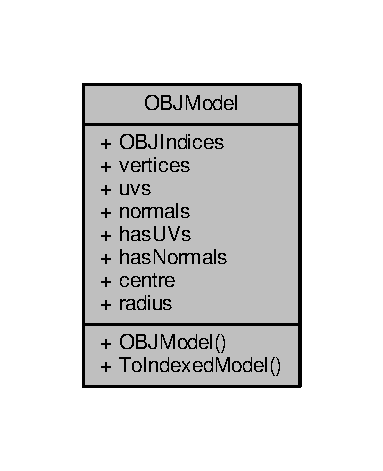
\includegraphics[width=184pt]{class_o_b_j_model__coll__graph}
\end{center}
\end{figure}
\subsection*{Public Member Functions}
\begin{DoxyCompactItemize}
\item 
{\bfseries O\+B\+J\+Model} (const std\+::string \&file\+Name)\hypertarget{class_o_b_j_model_ac33fd4d7e20cd7ca5a82962015e91686}{}\label{class_o_b_j_model_ac33fd4d7e20cd7ca5a82962015e91686}

\item 
\hyperlink{class_indexed_model}{Indexed\+Model} {\bfseries To\+Indexed\+Model} ()\hypertarget{class_o_b_j_model_ad1e4ca6919c26a164aca9fa83523f142}{}\label{class_o_b_j_model_ad1e4ca6919c26a164aca9fa83523f142}

\end{DoxyCompactItemize}
\subsection*{Public Attributes}
\begin{DoxyCompactItemize}
\item 
std\+::vector$<$ \hyperlink{struct_o_b_j_index}{O\+B\+J\+Index} $>$ {\bfseries O\+B\+J\+Indices}\hypertarget{class_o_b_j_model_a6522870686168e757385b62214abe37b}{}\label{class_o_b_j_model_a6522870686168e757385b62214abe37b}

\item 
std\+::vector$<$ glm\+::vec3 $>$ {\bfseries vertices}\hypertarget{class_o_b_j_model_aa1444e5c0ec8249988d5b7a1f54297c6}{}\label{class_o_b_j_model_aa1444e5c0ec8249988d5b7a1f54297c6}

\item 
std\+::vector$<$ glm\+::vec2 $>$ {\bfseries uvs}\hypertarget{class_o_b_j_model_a66d03d734db51477fce847066d472993}{}\label{class_o_b_j_model_a66d03d734db51477fce847066d472993}

\item 
std\+::vector$<$ glm\+::vec3 $>$ {\bfseries normals}\hypertarget{class_o_b_j_model_af61e5eb97529d47fe8e050fcd0bc976a}{}\label{class_o_b_j_model_af61e5eb97529d47fe8e050fcd0bc976a}

\item 
bool {\bfseries has\+U\+Vs}\hypertarget{class_o_b_j_model_a68c309623f6223858524180eac4c8dff}{}\label{class_o_b_j_model_a68c309623f6223858524180eac4c8dff}

\item 
bool {\bfseries has\+Normals}\hypertarget{class_o_b_j_model_a306f4792cc8b11ffdae23de05e299b07}{}\label{class_o_b_j_model_a306f4792cc8b11ffdae23de05e299b07}

\item 
glm\+::vec3 {\bfseries centre}\hypertarget{class_o_b_j_model_a6c135bd19ee5deda173082d907378cc0}{}\label{class_o_b_j_model_a6c135bd19ee5deda173082d907378cc0}

\item 
float {\bfseries radius}\hypertarget{class_o_b_j_model_a88559cdd84893f4e52b26cc51edeb3ee}{}\label{class_o_b_j_model_a88559cdd84893f4e52b26cc51edeb3ee}

\end{DoxyCompactItemize}


The documentation for this class was generated from the following files\+:\begin{DoxyCompactItemize}
\item 
obj\+\_\+loader.\+h\item 
obj\+\_\+loader.\+cpp\end{DoxyCompactItemize}

\hypertarget{class_shader}{}\section{Shader Class Reference}
\label{class_shader}\index{Shader@{Shader}}


Collaboration diagram for Shader\+:\nopagebreak
\begin{figure}[H]
\begin{center}
\leavevmode
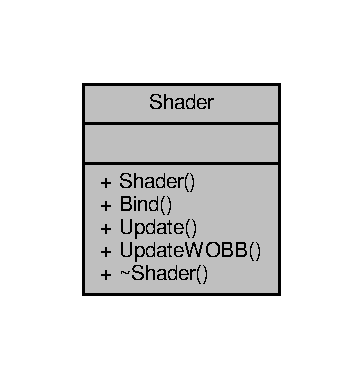
\includegraphics[width=174pt]{class_shader__coll__graph}
\end{center}
\end{figure}
\subsection*{Public Member Functions}
\begin{DoxyCompactItemize}
\item 
{\bfseries Shader} (const std\+::string \&file\+Name)\hypertarget{class_shader_a2c4961936691818dee95a5ef7c40155a}{}\label{class_shader_a2c4961936691818dee95a5ef7c40155a}

\item 
void {\bfseries Bind} ()\hypertarget{class_shader_a8b5c8c4788d011a65d158ef8428d1ece}{}\label{class_shader_a8b5c8c4788d011a65d158ef8428d1ece}

\item 
void {\bfseries Update} (\hyperlink{class_transform}{Transform} \&transform\+\_\+camera, const \hyperlink{class_camera}{Camera} \&camera, \hyperlink{class_transform}{Transform} \&transform\+\_\+mesh, \hyperlink{struct_material}{Material} material)\hypertarget{class_shader_ab1726c73d854211d8011afcfb157d5b7}{}\label{class_shader_ab1726c73d854211d8011afcfb157d5b7}

\item 
void {\bfseries Update\+W\+O\+BB} (const \hyperlink{class_transform}{Transform} \&transform\+\_\+camera, const \hyperlink{class_camera}{Camera} \&camera, const \hyperlink{class_transform}{Transform} \&transform\+\_\+\+O\+BB)\hypertarget{class_shader_af2504477df3226b64e65b0240ce45fd0}{}\label{class_shader_af2504477df3226b64e65b0240ce45fd0}

\end{DoxyCompactItemize}


The documentation for this class was generated from the following files\+:\begin{DoxyCompactItemize}
\item 
shader.\+h\item 
shader.\+cpp\end{DoxyCompactItemize}

\hypertarget{struct_silhouette_data}{}\section{Silhouette\+Data Struct Reference}
\label{struct_silhouette_data}\index{Silhouette\+Data@{Silhouette\+Data}}


Collaboration diagram for Silhouette\+Data\+:\nopagebreak
\begin{figure}[H]
\begin{center}
\leavevmode
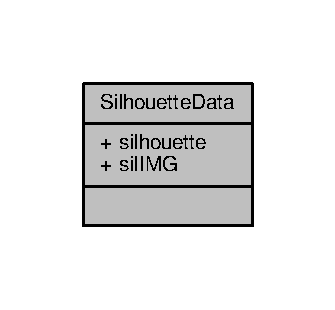
\includegraphics[width=161pt]{struct_silhouette_data__coll__graph}
\end{center}
\end{figure}
\subsection*{Public Attributes}
\begin{DoxyCompactItemize}
\item 
Silhouette {\bfseries silhouette}\hypertarget{struct_silhouette_data_a3d3e23a470900cc7833b7b9e07f1162b}{}\label{struct_silhouette_data_a3d3e23a470900cc7833b7b9e07f1162b}

\item 
cv\+::\+Mat {\bfseries sil\+I\+MG}\hypertarget{struct_silhouette_data_aa9b4629e5207c319e1cb56e2e3c89305}{}\label{struct_silhouette_data_aa9b4629e5207c319e1cb56e2e3c89305}

\end{DoxyCompactItemize}


The documentation for this struct was generated from the following file\+:\begin{DoxyCompactItemize}
\item 
similarityevaluator.\+h\end{DoxyCompactItemize}

\hypertarget{class_similarity_evaluator}{}\section{Similarity\+Evaluator Class Reference}
\label{class_similarity_evaluator}\index{Similarity\+Evaluator@{Similarity\+Evaluator}}


Collaboration diagram for Similarity\+Evaluator\+:
\nopagebreak
\begin{figure}[H]
\begin{center}
\leavevmode
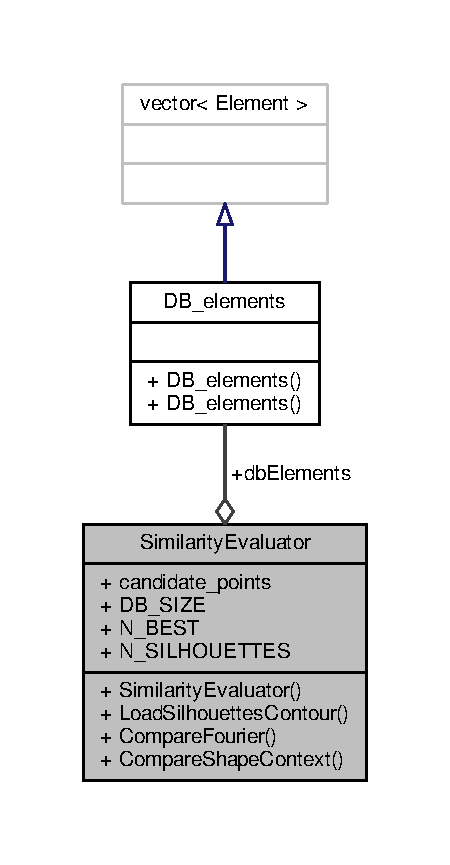
\includegraphics[width=216pt]{class_similarity_evaluator__coll__graph}
\end{center}
\end{figure}
\subsection*{Public Member Functions}
\begin{DoxyCompactItemize}
\item 
{\bfseries Similarity\+Evaluator} (\hyperlink{class_d_b__elements}{D\+B\+\_\+elements} \&elements, const int candidate\+\_\+points)\hypertarget{class_similarity_evaluator_af57882bf4c3246f8b0fc01762229da69}{}\label{class_similarity_evaluator_af57882bf4c3246f8b0fc01762229da69}

\item 
void {\bfseries Load\+Silhouettes\+Contour} ()\hypertarget{class_similarity_evaluator_af03cc295b586ccf9488679d6522de322}{}\label{class_similarity_evaluator_af03cc295b586ccf9488679d6522de322}

\item 
vector$<$ int $>$ {\bfseries Compare\+Fourier} ()\hypertarget{class_similarity_evaluator_a48db0709896d183332421205bdd0b414}{}\label{class_similarity_evaluator_a48db0709896d183332421205bdd0b414}

\item 
vector$<$ int $>$ {\bfseries Compare\+Shape\+Context} ()\hypertarget{class_similarity_evaluator_af6fca85ce5d1cb8f120860cbad197767}{}\label{class_similarity_evaluator_af6fca85ce5d1cb8f120860cbad197767}

\end{DoxyCompactItemize}
\subsection*{Public Attributes}
\begin{DoxyCompactItemize}
\item 
int {\bfseries candidate\+\_\+points}\hypertarget{class_similarity_evaluator_a7467ef9610c6a71aa0427029af1ed273}{}\label{class_similarity_evaluator_a7467ef9610c6a71aa0427029af1ed273}

\item 
int {\bfseries D\+B\+\_\+\+S\+I\+ZE}\hypertarget{class_similarity_evaluator_a36860f8a89407aced89f7af45889eeba}{}\label{class_similarity_evaluator_a36860f8a89407aced89f7af45889eeba}

\item 
const int {\bfseries N\+\_\+\+B\+E\+ST} = 3\hypertarget{class_similarity_evaluator_a2b1157b496d0bbe69955373df190b859}{}\label{class_similarity_evaluator_a2b1157b496d0bbe69955373df190b859}

\item 
const int {\bfseries N\+\_\+\+S\+I\+L\+H\+O\+U\+E\+T\+T\+ES} = 3\hypertarget{class_similarity_evaluator_a71a77ff07d798b82123d84727ec0abe0}{}\label{class_similarity_evaluator_a71a77ff07d798b82123d84727ec0abe0}

\item 
\hyperlink{class_d_b__elements}{D\+B\+\_\+elements} {\bfseries db\+Elements}\hypertarget{class_similarity_evaluator_a4e1e65229b89da6ceb29cfd0be1741cb}{}\label{class_similarity_evaluator_a4e1e65229b89da6ceb29cfd0be1741cb}

\end{DoxyCompactItemize}


The documentation for this class was generated from the following files\+:\begin{DoxyCompactItemize}
\item 
similarityevaluator.\+h\item 
similarityevaluator.\+cpp\end{DoxyCompactItemize}

\hypertarget{class_transform}{}\section{Transform Class Reference}
\label{class_transform}\index{Transform@{Transform}}


Collaboration diagram for Transform\+:\nopagebreak
\begin{figure}[H]
\begin{center}
\leavevmode
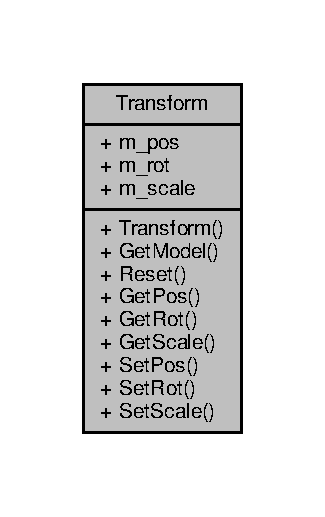
\includegraphics[width=156pt]{class_transform__coll__graph}
\end{center}
\end{figure}
\subsection*{Public Member Functions}
\begin{DoxyCompactItemize}
\item 
{\bfseries Transform} (const glm\+::vec3 \&pos=glm\+::vec3(), const glm\+::vec3 \&rot=glm\+::vec3(), const glm\+::vec3 \&scale=glm\+::vec3(1.\+0f, 1.\+0f, 1.\+0f))\hypertarget{class_transform_add035b5fd0670b28e001376e3bd0b3e4}{}\label{class_transform_add035b5fd0670b28e001376e3bd0b3e4}

\item 
glm\+::mat4 {\bfseries Get\+Model} () const \hypertarget{class_transform_a595794de4a147c89235954314f451581}{}\label{class_transform_a595794de4a147c89235954314f451581}

\item 
void {\bfseries Reset} ()\hypertarget{class_transform_a595f025127f8297ff0d159beb9c8fdd5}{}\label{class_transform_a595f025127f8297ff0d159beb9c8fdd5}

\item 
glm\+::vec3 \& {\bfseries Get\+Pos} ()\hypertarget{class_transform_aac3ae43f96c83f13326623c75939475b}{}\label{class_transform_aac3ae43f96c83f13326623c75939475b}

\item 
glm\+::vec3 \& {\bfseries Get\+Rot} ()\hypertarget{class_transform_afd30598557e0b9481d80c973d5f38966}{}\label{class_transform_afd30598557e0b9481d80c973d5f38966}

\item 
glm\+::vec3 \& {\bfseries Get\+Scale} ()\hypertarget{class_transform_ab1beb0c0174d15cd211625265c54e52c}{}\label{class_transform_ab1beb0c0174d15cd211625265c54e52c}

\item 
void {\bfseries Set\+Pos} (glm\+::vec3 \&pos)\hypertarget{class_transform_a7224aa5c71fe8c24f69503c92274c143}{}\label{class_transform_a7224aa5c71fe8c24f69503c92274c143}

\item 
void {\bfseries Set\+Rot} (glm\+::vec3 \&rot)\hypertarget{class_transform_ae90159b68dc95535b8c63eccce2a9ea1}{}\label{class_transform_ae90159b68dc95535b8c63eccce2a9ea1}

\item 
void {\bfseries Set\+Scale} (glm\+::vec3 \&scale)\hypertarget{class_transform_ae3fabfd2a2ff59c019f7ad2eefe16dae}{}\label{class_transform_ae3fabfd2a2ff59c019f7ad2eefe16dae}

\end{DoxyCompactItemize}
\subsection*{Public Attributes}
\begin{DoxyCompactItemize}
\item 
glm\+::vec3 {\bfseries m\+\_\+pos}\hypertarget{class_transform_a4fc3e74f53c30bfa44a96fbc4140b3f3}{}\label{class_transform_a4fc3e74f53c30bfa44a96fbc4140b3f3}

\item 
glm\+::vec3 {\bfseries m\+\_\+rot}\hypertarget{class_transform_a1828f07ae48b9afec249023cd9de8c78}{}\label{class_transform_a1828f07ae48b9afec249023cd9de8c78}

\item 
glm\+::vec3 {\bfseries m\+\_\+scale}\hypertarget{class_transform_aefc54a7741af00958612ed0f9596b702}{}\label{class_transform_aefc54a7741af00958612ed0f9596b702}

\end{DoxyCompactItemize}


The documentation for this class was generated from the following file\+:\begin{DoxyCompactItemize}
\item 
transform.\+h\end{DoxyCompactItemize}

\hypertarget{class_vertex}{}\section{Vertex Class Reference}
\label{class_vertex}\index{Vertex@{Vertex}}


Collaboration diagram for Vertex\+:\nopagebreak
\begin{figure}[H]
\begin{center}
\leavevmode
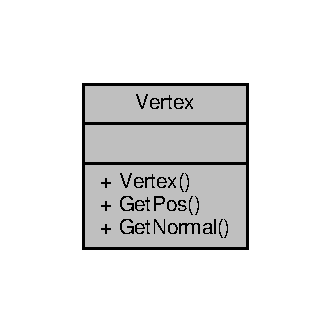
\includegraphics[width=159pt]{class_vertex__coll__graph}
\end{center}
\end{figure}
\subsection*{Public Member Functions}
\begin{DoxyCompactItemize}
\item 
{\bfseries Vertex} (const glm\+::vec3 \&pos, const glm\+::vec3 \&normal=glm\+::vec3(0, 0, 0))\hypertarget{class_vertex_ad575d03337b04df7b54f992a3b5431b0}{}\label{class_vertex_ad575d03337b04df7b54f992a3b5431b0}

\item 
glm\+::vec3 $\ast$ {\bfseries Get\+Pos} ()\hypertarget{class_vertex_a2b1f942f9af5b03144bd92b9ca115aea}{}\label{class_vertex_a2b1f942f9af5b03144bd92b9ca115aea}

\item 
glm\+::vec3 $\ast$ {\bfseries Get\+Normal} ()\hypertarget{class_vertex_ab8137faa3c736fd97e400b4f75750900}{}\label{class_vertex_ab8137faa3c736fd97e400b4f75750900}

\end{DoxyCompactItemize}


The documentation for this class was generated from the following file\+:\begin{DoxyCompactItemize}
\item 
mesh.\+h\end{DoxyCompactItemize}

%--- End generated contents ---

% Index
\backmatter
\newpage
\phantomsection
\clearemptydoublepage
\addcontentsline{toc}{chapter}{Index}
\printindex

\end{document}
